%\documentclass[xcolor=table,handout,compress]{beamer}
\documentclass[xcolor=table]{beamer}

%--------------------------------------------------------------------------
% Common packages
%--------------------------------------------------------------------------
\usepackage[english]{babel}
\usepackage{pgfpages} % required for notes on second screen
\usepackage{graphicx}
\usepackage{subfigure}
\usepackage{multicol}
\usepackage[normalem]{ulem}

\usepackage{tabularx,ragged2e}
\usepackage{booktabs}
\usepackage{marvosym}

\makeatletter
\let\beamer@writeslidentry@miniframeson=\beamer@writeslidentry
\def\beamer@writeslidentry@miniframesoff{%
  \expandafter\beamer@ifempty\expandafter{\beamer@framestartpage}{}% does not happen normally
  {%else
    % removed \addtocontents commands
    \clearpage\beamer@notesactions%
  }
}
\newcommand*{\miniframeson}{\let\beamer@writeslidentry=\beamer@writeslidentry@miniframeson}
\newcommand*{\miniframesoff}{\let\beamer@writeslidentry=\beamer@writeslidentry@miniframesoff}
\makeatother


%--------------------------------------------------------------------------
% Load theme
%--------------------------------------------------------------------------
\usetheme{hri}

\usepackage{tikz}
\usetikzlibrary{patterns,shapes,fpu,fit,calc,mindmap,backgrounds,positioning,svg.path}

\tikzset{
  invisible/.style={opacity=0},
  visible on/.style={alt={#1{}{invisible}}},
  alt/.code args={<#1>#2#3}{%
    \alt<#1>{\pgfkeysalso{#2}}{\pgfkeysalso{#3}} % \pgfkeysalso doesn't change the path
  },
}

%% Neat trick to have only one navigation bullet per subsection
%% http://tex.stackexchange.com/questions/64333/one-navigation-bullet-per-subsection-with-subsection-false-in-custom-beamer-them
%\usepackage{etoolbox}
%\makeatletter
%\patchcmd{\slideentry}{\advance\beamer@xpos by1\relax}{}{}{}
%\def\beamer@subsectionentry#1#2#3#4#5{\advance\beamer@xpos by1\relax}%
%\makeatother
%%%%%%%%%%%%%%%%%%%%%%%%%%%%%%%%%%%%%%%

\graphicspath{{figs/}}

% for model of anthopomorphism
\newcommand{\IPA}{{$\mathcal{A}_0$~}}
\newcommand{\SLA}{{$\mathcal{A}_\infty$~}}
\newcommand{\sla}{{\mathcal{A}_\infty}}
\newcommand{\AntMax}{{$\mathcal{A}_{max}$~}}
\newcommand{\antMax}{{\mathcal{A}_{max}}}

% for HATP plans
\newcommand{\hatpaction}[3]{#1\\\textsf{\scriptsize #2,}\\\textsf{\scriptsize #3}}
\newcommand{\stmt}[1]{{\footnotesize \tt  #1}}

% for mutual modelling
\newcommand{\Mmodel}[3]{{\mathcal{M}(#1, #2, #3)}}
\newcommand{\model}[3]{{$\mathcal{M}(#1, #2, #3)$}}
\newcommand{\Model}[3]{{$\mathcal{M}^{\circ}(#1, #2, #3)$}}

% typeset logical concept
\newcommand{\concept}[1]{{\scriptsize \texttt{#1}}}

\newcommand{\backbutton}{\hfill\hyperlink{appendix}{\beamerreturnbutton{Supplementary material}}}
%--------------------------------------------------------------------------
% General presentation settings
%--------------------------------------------------------------------------
\title{cognition \& HRI}
\subtitle{how to \emph{do} together?}
\date{{\bf  UKRAS19} -- 24th Jan. 2019}
\author{Séverin Lemaignan}
\institute{{\bf Bristol Robotics Lab} University of the West of England}

%--------------------------------------------------------------------------
% Notes settings
%--------------------------------------------------------------------------
%\setbeameroption{show notes on second screen}
%\setbeameroption{hide notes}

\begin{document}


%%%%%%%%%%%%%%%%%%%%%%%%%%%%%%%%%%%%%%%%%%%%%%%%%%%%%%%%


%%%%%%%%%%%%%%%%%%%%%%%%%%%%%%%%%%%%%%%%%%%%%%%%%%%%%%%%


%%%%%%%%%%%%%%%%%%%%%%%%%%%%%%%%%%%%%%%%%%%%%%%%%%%%%%%%

\maketitle

%%%%%%%%%%%%%%%%%%%%%%%%%%%%%%%%%%%%%%%%%%%%%%%%%%%%%%%%

\licenseframe{github.com/severin-lemaignan/l2tor-symposium2018-technical-challenges-cri}

%%%%%%%%%%%%%%%%%%%%%%%%%%%%%%%%%%%%%%%%%%%%%%%%%%%%%%%%

{
    \paper{Lemaignan et al. {\bf Artificial Cognition for Social Human-Robot
    Interaction: An Implementation} Artificial Intelligence 2017}
\begin{frame}{Model-based joint action}
    \badge{laas}
    \begin{enumerate}
        \item establish a joint goal
        \item plan for the robot
        \item plan for the human in order to build a set of priors
        \item execute the robot plan
        \item monitor progress of the partner towards the goal
    \end{enumerate}

    \pause

    $\Rightarrow$ {\bf explicit cognitive steps}
    \pause

    \emph{...hard ones, though:
    \begin{itemize}
        \item how to communicate/agree on goals \& plans?
        \item what about the human's own plans?
        \item monitoring/recognising error situations
        \item what to do when we're going 'off track'?
        \item ...
    \end{itemize}
    }

\end{frame}
}

%%%%%%%%%%%%%%%%%%%%%%%%%%%%%%%%%%%%%%%%%%%%%%%%%%%%%%%%

{
    \paper{Lemaignan et al. {\bf Artificial Cognition for Social Human-Robot
    Interaction: An Implementation} -- Artificial Intelligence 2017}

\begin{frame}{We can do a bit already}

    \begin{center}
    \only<1>{
            \video{0.9\columnwidth}{figs/perspective-taking/this_box.webm?start=1}
        }
        \only<2>{
            \video{0.9\columnwidth}{figs/underworlds/underworlds.mp4?start=20}
        }
    \end{center}

    \badge{laas}
\end{frame}

}

%%%%%%%%%%%%%%%%%%%%%%%%%%%%%%%%%%%%%%%%%%%%%%%%%%%%%%%%

\begin{frame}{How do humans perform tasks together?}


    \begin{center}
        {\bf Collaborating is a costly socio-cognitive activity}.

    \pause
    Humans are good at it.
        
    They are also really good at minimizing the cost
    involved.
    \pause
    
        The key mechanism: {\bf prefer implicit to explicit}

    \pause

        ...which is closely related to: {\bf be lazy}
        
        First, go for the simple -- if possibly ambiguous -- actions; and, if
        really needed, repair

    \pause
    \vspace{2cm}
    {\bf What does ``be lazy'' mean for robots?}
    \end{center}
        
\end{frame}

%%%%%%%%%%%%%%%%%%%%%%%%%%%%%%%%%%%%%%%%%%%%%%%%%%%%%%%%

\begin{frame}{One example: grounding of spatial language}


    \begin{center}
        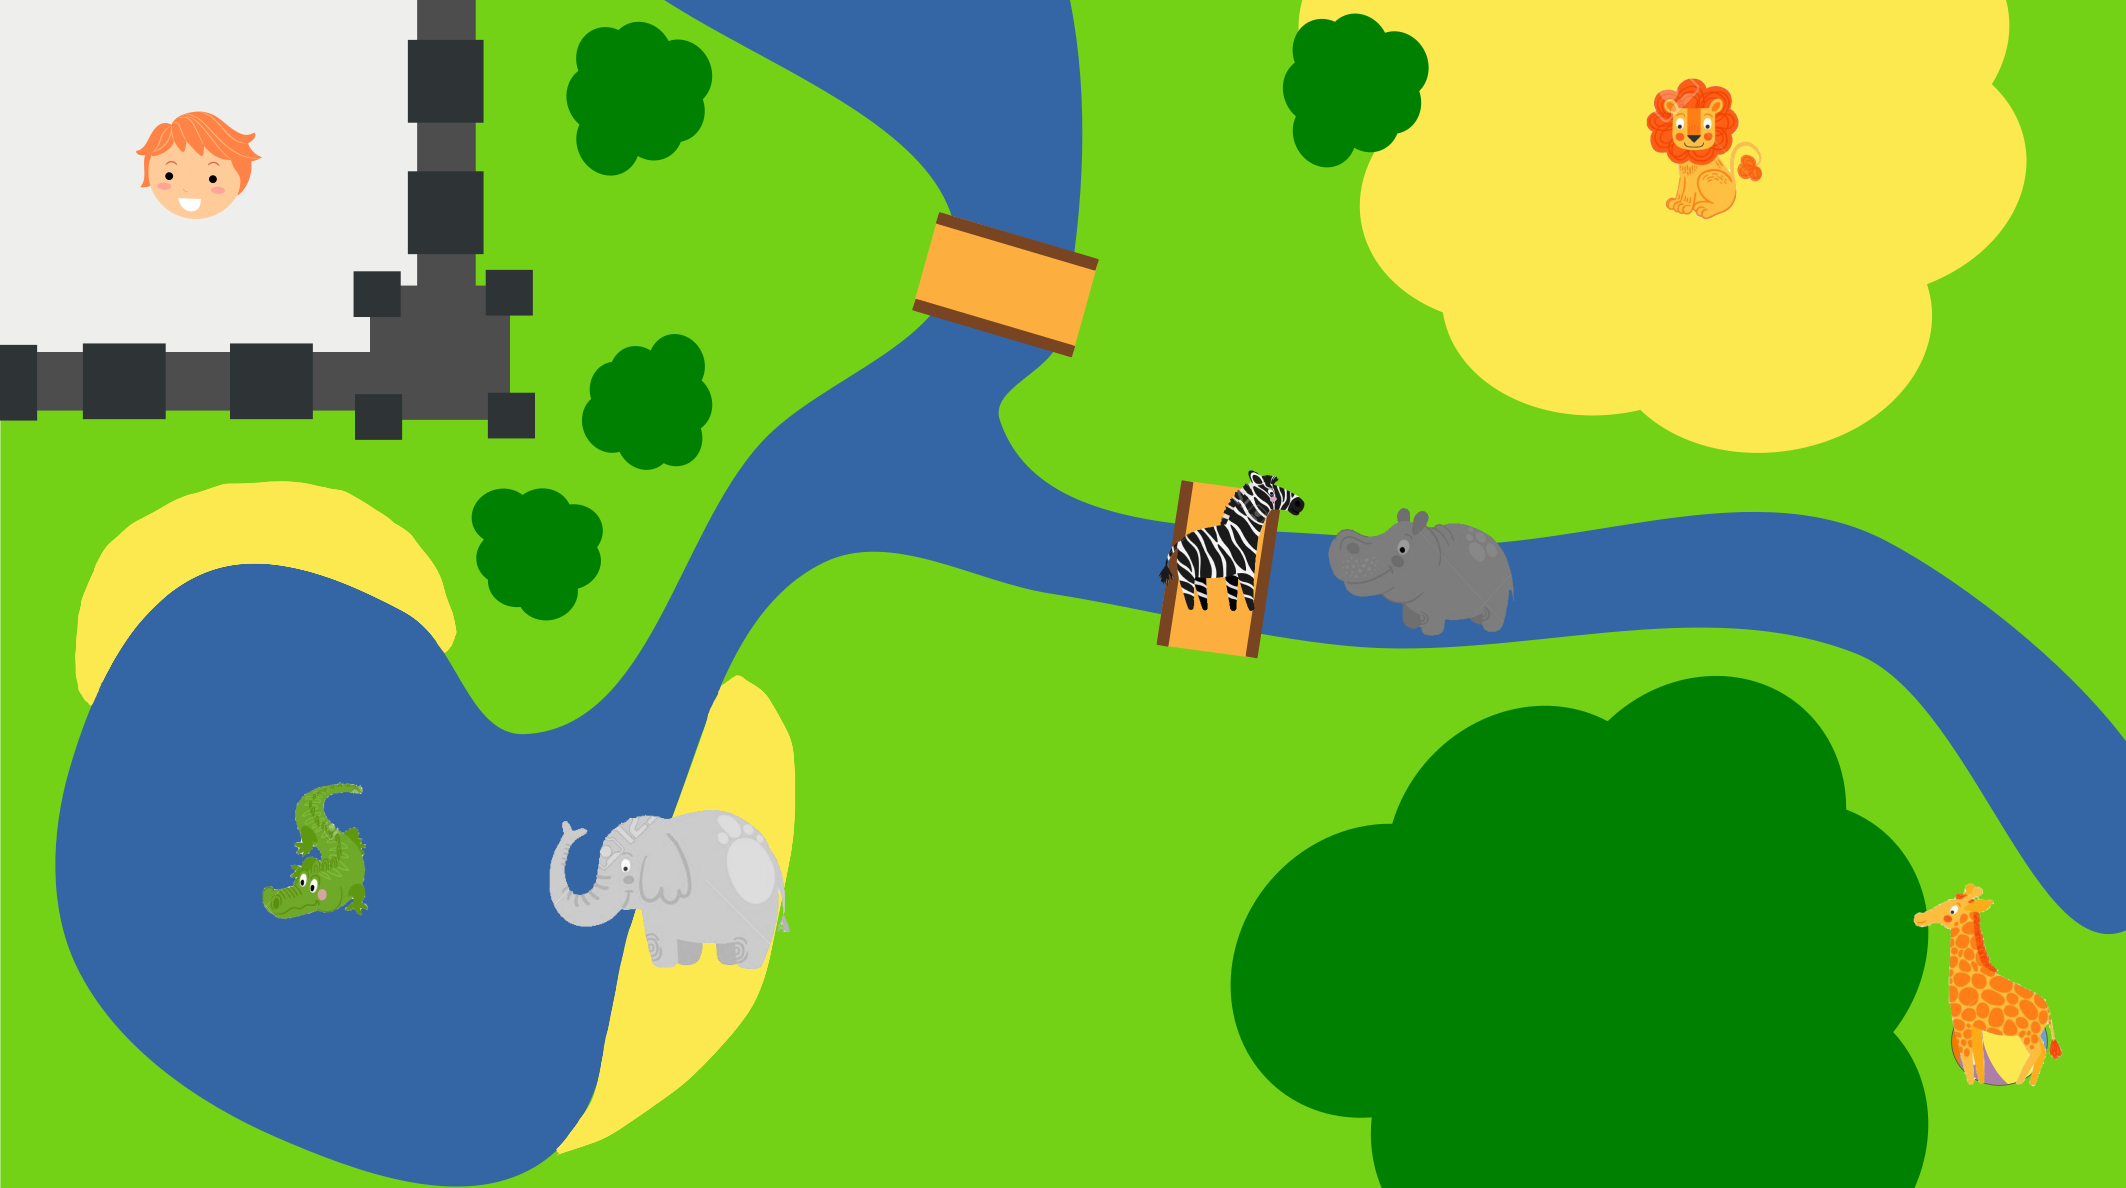
\includegraphics[width=0.9\linewidth]{ambiguous-desc/RefMap}

    Ambiguities arise easily when describing spatial scenes.

    How do we solve them?

    \end{center}

    \badge{chris}
\end{frame}

%%%%%%%%%%%%%%%%%%%%%%%%%%%%%%%%%%%%%%%%%%%%%%%%%%%%%%%%

\imageframe[color=black]{ambiguous-desc/NosePointCropped}

%%%%%%%%%%%%%%%%%%%%%%%%%%%%%%%%%%%%%%%%%%%%%%%%%%%%%%%%

\imageframe{ambiguous-desc/LanguageUse}

%%%%%%%%%%%%%%%%%%%%%%%%%%%%%%%%%%%%%%%%%%%%%%%%%%%%%%%%

{\paper{Clark and Wilkes-Gibbs, \emph{Referring as a collaborative
process}, Cognition 1986 \newline Pickering and Garrod, \emph{Alignment as the basis for successful
communication}, Research on Language and Computation 2006}
\begin{frame}{surface alignment; grounding criterion}

    Psycholinguistics provides a lot of the foundational work on these
    questions.

    \begin{itemize}
        \item<+-> \emph{Communication is a dynamic social process}: the partner often to signal
            missing/misunderstood informations
        \item<+-> Repairing is generally less costly than avoiding ambiguities in
            the first place
        \item<+-> You only ever need to reach the \emph{grounding criterion}, ie
            \emph{enough} mutual understanding for the task
        \item<+-> $\Rightarrow$ we typically only reach \emph{partial (or surface)
            alignment} -- full alignment is usually not required
        %\item<+-> {\bf do we need a high-level Theory of Mind at all?}
    \end{itemize}
\end{frame}
}

%%%%%%%%%%%%%%%%%%%%%%%%%%%%%%%%%%%%%%%%%%%%%%%%%%%%%%%%

\begin{frame}{In social Human-Robot interaction}

    \only<1>{
        Well studied in communication (cf back-channeling)

    Can we expand this line of thought to sHRI in general?

    Most of our social and behavioural alignment comes from sub-conscious social
    mechanisms:

    \begin{itemize}
        \item entrainment (coupling), 
        \item mimicry, 
        \item implicit turn-taking,
        \item joint attention
        \item ...and others
    \end{itemize}
    \pause
    \begin{center}
        Can we model \& generate them?
    \end{center}

}

    \only<2>{
        \begin{itemize}
            \item These mechanisms are unfortunately often ill-defined, and
                particularly difficult to turn into equations (or controllers, in
                our case)
            \item no close-form equation of social interactions $\Rightarrow$ data-driven approaches?
        \end{itemize}
    }
\end{frame}

%%%%%%%%%%%%%%%%%%%%%%%%%%%%%%%%%%%%%%%%%%%%%%%%%%%%%%%%
%%%%%%%%%%%%%%%%%%%%%%%%%%%%%%%%%%%%%%%%%%%%%%%%%%%%%%%%

\section[Data-driven!]{Towards the data-driven study of social dynamics}

%%%%%%%%%%%%%%%%%%%%%%%%%%%%%%%%%%%%%%%%%%%%%%%%%%%%%%%%

\begin{frame}{Data!}

    If we want to use machine learning, we need data (relevant to child-robot
    interactions in a learning environment).
    
    \pause

    ...a task that exhibits:

    \begin{itemize}
        \item complex social dynamics
        \item open, underspecified situations
        \item natural interactions
        \item rich semantics
        \item interplay of many socio-cognitive functions
    \end{itemize}

    \pause

    while being...
    \begin{itemize}
        \item reproducible/replicable experimental procedure
        \item clear quantitative metrics
        \item practical
    \end{itemize}
\end{frame}

%%%%%%%%%%%%%%%%%%%%%%%%%%%%%%%%%%%%%%%%%%%%%%%%%%%%%%%%

\begin{frame}{Free play}

    \begin{center}
    {\Large ``Just play! Enjoy yourselves!''}
    \end{center}

    \vspace{3em}

    \begin{itemize}
        \item \textbf{rich set of cognitive and
            social dynamics}; importance of motivation/drive; \textbf{uncertain
            and unexpected situations}
        \item what is the right action policy? Focus instead on the \textbf{social policy}
    \end{itemize}
    \pause
    \begin{itemize}
        \item focus on children
        \item with a little bit of scaffolding \& framing
    \end{itemize}


\end{frame}

%%%%%%%%%%%%%%%%%%%%%%%%%%%%%%%%%%%%%%%%%%%%%%%%%%%%%%%%

\imageframe{freeplay/freeplay-overview2}

%%%%%%%%%%%%%%%%%%%%%%%%%%%%%%%%%%%%%%%%%%%%%%%%%%%%%%%%

\begin{frame}{Freeplay sandox in a nutshell}

    A task that exhibits...

    \begin{itemize}
        \item open, underspecified situations
            \item complex social dynamics
            \item natural interactions
            \item rich semantics
            \item interplay of many socio-cognitive functions
    \end{itemize}

    \pause

    while being...
    \begin{itemize}
        \item reproducible/replicable experimental procedure
        \item clear quantitative metrics
        \item practical
    \end{itemize}
\end{frame}


\begin{frame}{Social dynamics to be observed}

    \begin{itemize}
        \item<+-> the \textbf{task engagement}
            \begin{itemize}
                \item are the participants 'on task' or not?
            \end{itemize}
        \item<+-> the \textbf{interaction flow} \& \textbf{situation awareness}
            \begin{itemize}
                \item what is happening \emph{now}? what is the next expected
                    action?
            \end{itemize}
        \item<+-> the \textbf{social attitude}
            \begin{itemize}
                \item pro-social, hostile, assertive (‘bossy’), passive...
            \end{itemize}
        \item<+-> the \textbf{social dynamics}
            \begin{itemize}
                \item entrainment (coupling), mimicry, implicit turn-taking, joint
                    attention
            \end{itemize}
    \end{itemize}

    \pause
    $\rightarrow$ {\bf paradigm for socio-cognitive investigation}
\end{frame}




{
    \paper{Lemaignan et al. {\bf The PInSoRo
    dataset: Supporting the data-driven study of [...]} PLOS One 2018}
\begin{frame}{The PInSoRo dataset}
    \begin{itemize}
        \item 120 children, 4 to 8 years old
        \item 75 interactions
            \begin{itemize}
                \item 90 children playing with another child, 
                \item 30 playing with a robot
            \end{itemize}
        \item About 45h+ of recordings; 2M+ frames; $\approx$ 2TB
         \item average duration of freeplay interactions: 24min in child-child
         condition; 19min in child-robot condition
    \end{itemize}

\end{frame}
}

\videoframe[0.56]{figs/pinsoro/optical_flow.mp4?autostart}

%%%%%%%%%%%%%%%%%%%%%%%%%%%%%%%%%%%%%%%%%%%%%%%%%%%%%%%%

\begin{frame}{13000+ annotations}
    \begin{center}
        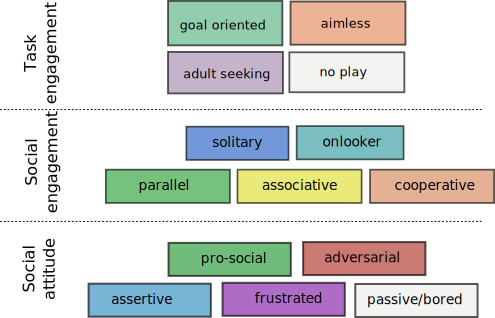
\includegraphics[width=0.8\linewidth]{freeplay/coding-scheme}
    \end{center}
\end{frame}

%%%%%%%%%%%%%%%%%%%%%%%%%%%%%%%%%%%%%%%%%%%%%%%%%%%%%%%%
\begin{frame}{Two baselines}

    \begin{center}
        \includegraphics<1>[width=\linewidth]{pinsoro/pinsoro-baselines}
        \includegraphics<2>[width=\linewidth]{pinsoro/pinsoro-baselines2}
    \end{center}
\end{frame}


%%%%%%%%%%%%%%%%%%%%%%%%%%%%%%%%%%%%%%%%%%%%%%%%%%%%%%%%


%%%%%%%%%%%%%%%%%%%%%%%%%%%%%%%%%%%%%%%%%%%%%%%%%%%%%%%%

\videoframe[0.56]{figs/pinsoro/pinsoro-matplotlib.mp4?autostart}

\begin{frame}{Largest open dataset of natural social interactions}
    \Large
    \begin{center}
        \vspace{1cm}
        Anonymised version (7.2GB) available on-line. Grab it now!

        \LARGE \href{https://freeplay-sandbox.github.io}{\bf freeplay-sandbox.github.io}

        \vspace{1cm}
            \large Open data! Hosted on EU's  
\includegraphics[width=0.3\linewidth]{zenodo}
    \end{center}
\end{frame}

%%%%%%%%%%%%%%%%%%%%%%%%%%%%%%%%%%%%%%%%%%%%%%%%%%%%%%%%

\section{Mining the data}

\videoframe[0.56]{figs/kinematics_social_dynamics/clip_skel_01.mp4}

%%%%%%%%%%%%%%%%%%%%%%%%%%%%%%%%%%%%%%%%%%%%%%%%%%%%%%%%

\videoframe[0.56]{figs/kinematics_social_dynamics/clip_01.mp4}

%%%%%%%%%%%%%%%%%%%%%%%%%%%%%%%%%%%%%%%%%%%%%%%%%%%%%%%%

\videoframe[0.56]{figs/kinematics_social_dynamics/clip_skel_05.mp4}

%%%%%%%%%%%%%%%%%%%%%%%%%%%%%%%%%%%%%%%%%%%%%%%%%%%%%%%%

\videoframe[0.56]{figs/kinematics_social_dynamics/clip_05.mp4}

\imageframe[caption={200 participants, 4 clips each, on MTurk}]{kinematics_social_dynamics/questionnaire.png}
\imageframe{kinematics_social_dynamics/dataset.png}
\imageframe[caption={For each construct, calculate $\Delta$ and $\Sigma$}]{kinematics_social_dynamics/dataset-sumdiff.png}

{
    \paper{Bartlett et al. \textbf{What Can You See? Identifying Cues on
Internal States from the Kinematics [...]} Frontiers
2019 \emph{(under review)}}

\begin{frame}{EFA: Exploratory Factor Analysis}

\tiny
\rowcolors{2}{gray!25}{white}
\begin{tabular}{lrr|rr|rr}

    {} & \multicolumn{2}{l}{\bf Factor 1\onslide<2->{: imbalance}} &
    \multicolumn{2}{l}{\bf Factor 2\onslide<2->{: (negative) valence}} & \multicolumn{2}{l}{\bf
    Factor 3\onslide<2->{: engagement}} \\
    {} & \emph{full-scene} &  \onslide<3->{\emph{mov.-alone}} & \emph{full-scene} &
    \onslide<3->{\emph{mov.-alone}} & \emph{full-scene} &
    \onslide<3->{\emph{mov.-alone}} \\
\midrule
    \textbf{$\Delta$ Sad       } &      0.41 &  \only<3->{0.52} &           &                  &           &       \\
    \textbf{$\Sigma$ Sad       } &           &                  &      0.72 & \only<3->{ 0.53} &           & \only<3->{ 0.49} \\
    \textbf{$\Delta$ Happy     } &      0.49 &  \only<3->{0.53} &           &                  &           & \\
    \textbf{$\Sigma$ Happy      } &           &                 &           & \only<3->{-0.51} &     -0.55 & \\
    \textbf{$\Delta$ Angry     } &      0.40 &  \only<3->{0.62} &           &                  &           & \\
    \textbf{$\Sigma$ Angry      } &           &                 &      0.81 & \only<3->{ 0.85} &           & \\
    \textbf{$\Delta$ Excited   } &      0.53 &  \only<3->{0.63} &           &                  &           & \\
    \textbf{$\Sigma$ Excited    } &           &                 &           &                  &     -0.71 & \\
    \textbf{$\Delta$ Calm      } &      0.45 &  \only<3->{0.63} &           &                  &           & \\
    \textbf{$\Sigma$ Calm       } &           &  \only<3-> {  } &           & \only<3->{-0.45} &           & \\
    \textbf{$\Delta$ Friendly  } &      0.69 &  \only<3->{0.56} &           &                  &           & \\
    \textbf{$\Sigma$ Friendly   } &           &  \only<3->{   } &           & \only<3->{-0.60} &     -0.43 & \\
    \textbf{$\Delta$ Aggressive} &      0.78 &  \only<3->{0.79} &           &                  &           & \\
    \textbf{$\Sigma$ Aggressive } &           &  \only<3->{   } &      0.80 & \only<3->{ 0.72} &     -0.36 & \\
    \textbf{$\Delta$ Engaged   } &           &  \only<3->{0.39} &           &                  &      0.65 & \only<3->{ 0.52} \\
    \textbf{$\Sigma$ Engaged    } &           &  \only<3->{   } &           &                  &     -0.64 & \only<3->{-0.64} \\
    \textbf{$\Delta$ Distracted} &           &  \only<3->{    } &           &                  &      0.65 & \only<3->{ 0.63} \\
    \textbf{$\Sigma$ Distracted } &           &  \only<3->{   } &      0.63 &                  &           & \only<3->{ 0.82} \\
    \textbf{$\Delta$ Bored     } &           &  \only<3->{0.44} &           &                  &      0.61 & \only<3->{ 0.54} \\
    \textbf{$\Sigma$ Bored      } &           &  \only<3->{   } &      0.58 &                  &      0.48 & \only<3->{ 0.83} \\
    \textbf{$\Delta$ Frustrated} &      0.53 &  \only<3->{0.61} &           &                  &           &       \\
    \textbf{$\Sigma$ Frustrated } &           &  \only<3->{   } &      0.70 & \only<3->{ 0.69} &           &       \\
    \textbf{$\Delta$ Dominant  } &      0.75 &  \only<3->{0.81} &           &                  &           &       \\
    \textbf{$\Sigma$ Dominant   } &           &  \only<3->{   } &      0.53 & \only<3->{ 0.52} &           &       \\
    \textbf{$\Delta$ Submissive} &      0.68 &  \only<3->{0.72} &           &                  &           &       \\
    \textbf{$\Sigma$ Submissive } &          &                  &      0.54 &                  &           &       \\

\end{tabular}

    \note{Very strong correlation: Factor 1: r = 0.94, p < 0.001; for Factor 2: r = 0.84, p < 0.001; for Factor 3: r = 0.81, p < 0.001}

\end{frame}
}

\begin{frame}{Three constructs to rule them all}
        \centering
        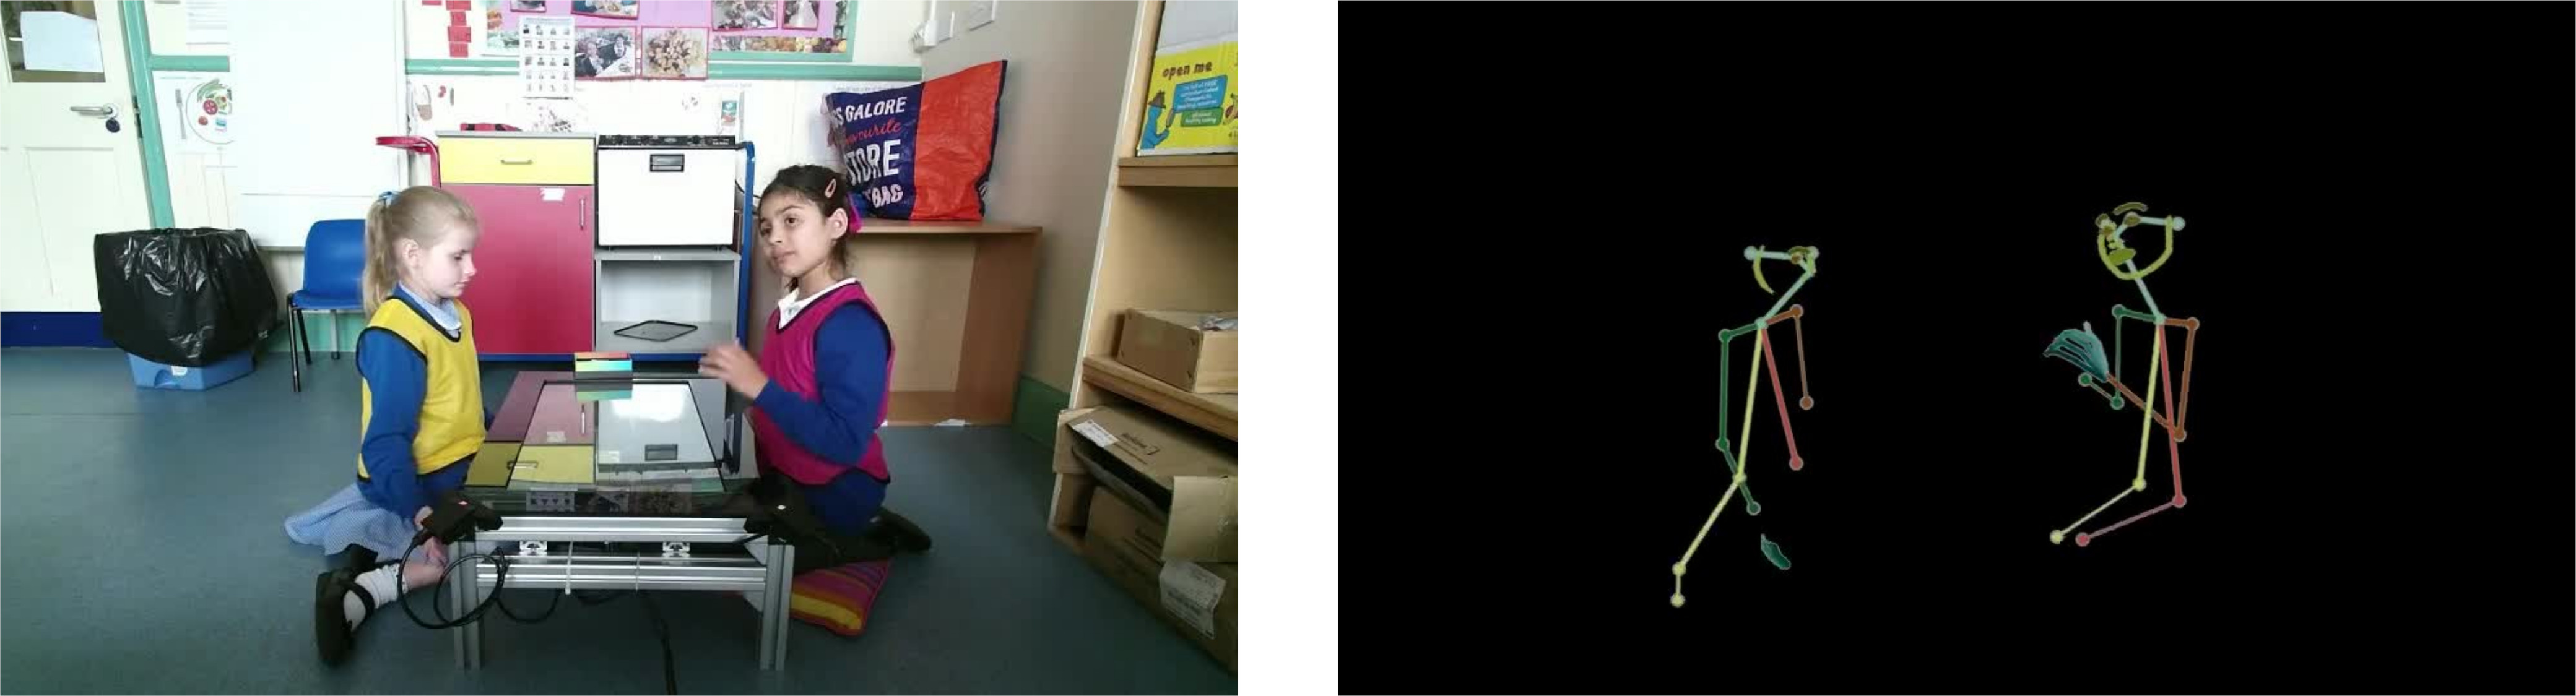
\includegraphics[width=0.9\linewidth]{kinematics_social_dynamics/clips.jpg}

    \textbf{Interaction imbalance}
    
    \textbf{Interaction valence}
    
    \textbf{Engagement}

\end{frame}

%%%%%%%%%%%%%%%%%%%%%%%%%%%%%%%%%%%%%%%%%%%%%%%%%%%%%%%%
\section[DNNs for Social Robotics]{Deep learning of social interactions?}

\videoframe[0.56]{figs/pinsoro/annotations.mp4?autostart}

\begin{frame}{Ultimately...}

    {\bf Real-time identification} by the robot of...

    \begin{itemize}
        \item<+-> the \textbf{task engagement}
            \begin{itemize}
                \item is my partner 'on task' or not?
            \end{itemize}
        \item<+-> the \textbf{interaction flow} \& \textbf{situation awareness}
            \begin{itemize}
                \item what is happening right now? should I do something?
            \end{itemize}
        \item<+-> the \textbf{social attitude}
            \begin{itemize}
                \item Pro-social, hostile, assertive (‘bossy’), passive...
            \end{itemize}
        \item<+-> the \textbf{social dynamics}
            \begin{itemize}
                \item entrainment (coupling), mimicry, turn-taking, joint
                    attention
            \end{itemize}
    \end{itemize}

    \pause

    Social behaviours; Social dynamics: \textbf{generation as well!}
\end{frame}

%%%%%%%%%%%%%%%%%%%%%%%%%%%%%%%%%%%%%%%%%%%%%%%%%%%%%%%%

\begin{frame}{What does that mean for CRI \& learning?}

    \begin{columns}
        \begin{column}{0.4\linewidth}
            
            \begin{center}
                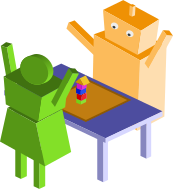
\includegraphics[width=0.9\linewidth]{joint-action-scenario-completed}
            \end{center}
        \end{column}
        \begin{column}{0.6\linewidth}
            \only<1-4> {
            \begin{itemize}
                \item<+-> We can reduce the socio-cognitive cost of
                    collaboration by relying as much
                    as possible on {\bf implicit (sub-conscious) social mechanisms}
                \item<+-> (do not be scared of ambiguous/partially defined
                    instructions/situations)
                \item<+-> The robot needs to learn to recognise and interpret
                    those social cues, hidden within complex social dynamics (in
                    real-time!)
                \item<+-> We have some raw material. Time to
                    process it together!
            \end{itemize}
        }
%            \only<5-> {
%            \begin{itemize}
%                \item<+-> Yet, {\bf learning does require cognitive effort \&
%                    engagement}. We simply want to direct it to the right
%                    subject.
%            \end{itemize}
%        }
%
        \end{column}
    \end{columns}
\end{frame}

%%%%%%%%%%%%%%%%%%%%%%%%%%%%%%%%%%%%%%%%%%%%%%%%%%%%%%%%

{
    \fullbackground[color=white]{c-r-t-succeed-dim}
\begin{frame}[plain]

    {\Large In summary:}

    \begin{itemize}
        \item<+-> Integration of \emph{social} robots in the classroom environment?
        \item<+-> Role of the teacher? \emph{Transfer of autonomy} looks like a
            promising lead.
        \item<+-> \emph{Doing together} with the child will require a better
            understanding of the social dynamics. Machine learning to the
            rescue?
        \item<+-> ...but the old assumption that full grounding of the
            communication is necessary, does not hold.
    \end{itemize}
\end{frame}
}

%%%%%%%%%%%%%%%%%%%%%%%%%%%%%%%%%%%%%%%%%%%%%%%%%%%%%%%%

{
    \fullbackground[color=white]{c-r-t-succeed-dim}
\begin{frame}[plain]

    {\Large Two open questions for the aspiring PhDs:}

    \begin{itemize}
        \item<+-> What about group dynamics?
        \item<+-> Over time, what place would a social robot take in the
            classroom?
    \end{itemize}
\end{frame}
}

%%%%%%%%%%%%%%%%%%%%%%%%%%%%%%%%%%%%%%%%%%%%%%%%%%%%%%%%

{
    \fullbackground[color=white]{c-r-t-succeed}
\begin{frame}[plain]

    \begin{columns}
        \begin{column}{0.5\linewidth}
        \vspace{4cm}

        \includegraphics[width=0.3\linewidth]{ayberk}
        \hspace{0.1cm}
        \includegraphics[width=0.3\linewidth]{deana}

        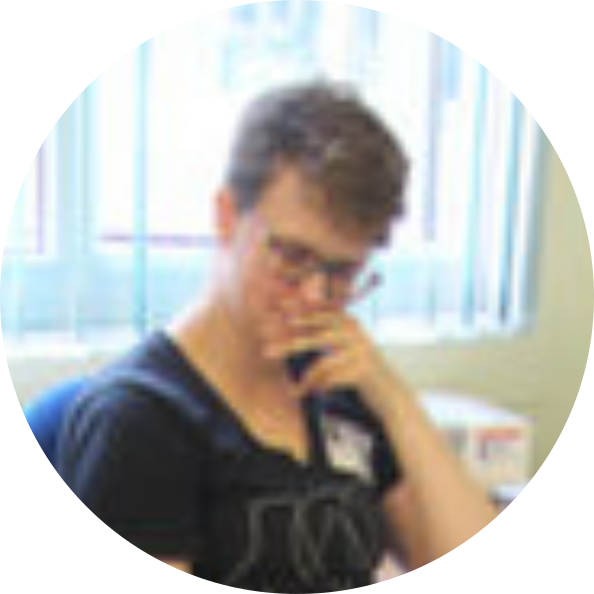
\includegraphics[width=0.3\linewidth]{charlotte}
        \hspace{0.1cm}
        
\includegraphics[width=0.3\linewidth]{emmanuel}

        
\includegraphics[width=0.3\linewidth]{chris}
        \hspace{0.1cm}
        
\includegraphics[width=0.3\linewidth]{maddy}

        \end{column}
        \begin{column}{0.5\linewidth}

    \vspace{6cm}
\setbeamercolor{hriSec1Demo}{fg=white!30!black}
\begin{beamercolorbox}[wd=\linewidth,ht=6ex,dp=0.7ex]{hriSec1Demo}
    \textbf{Thank you!}

\end{beamercolorbox}
        \end{column}
    \end{columns}
\end{frame}
}

%%%%%%%%%%%%%%%%%%%%%%%%%%%%%%%%%%%%%%%%%%%%%%%%%%%%%%%%

\section[]{Some more stuff}

%%%%%%%%%%%%%%%%%%%%%%%%%%%%%%%%%%%%%%%%%%%%%%%%%%%%%%%%

\begin{frame}{Some building blocks exists}

    \begin{itemize}
        \item \textbf{Multi-modal fusion}

            \begin{itemize}
                \item \eg Noda et al. {\bf Multimodal integration learning of robot behavior
    using DNN}, Robotics and Autonomous Systems 2014
            \end{itemize}

        \item \textbf{Behavioural sequences recognition}
            \begin{itemize}
                \item How et al. {\bf Behavior recognition for humanoid
                    robots using long short-term memory},
                    IJARS 2016 \emph{$\rightarrow$ LSTM to recognise Nao
                    behaviours}
                \item Shiarlis et al. {\bf Acquiring Social Interaction
                    Behaviours for Telepresence Robots via Deep Learning from
                    Demonstration}, IROS 2017
            \end{itemize}
    \end{itemize}

    \pause
    {\bf DBSoC: Deep Behavioural Social Cloning} -- LfD + CNNs + LSTM

    Two tasks for a telepresence robot:
    \begin{enumerate}
        \item position itself in a (dynamic) group of persons
        \item follow 2 persons
    \end{enumerate}
\end{frame}

%%%%%%%%%%%%%%%%%%%%%%%%%%%%%%%%%%%%%%%%%%%%%%%%%%%%%%%%

{
    \paper{taken from a NIPS2015 tutorial by Geoff Hinton, Yoshua Bengio \&
    Yann LeCun}

\begin{frame}{Deep networks $\equiv$ black boxes?}

    \begin{center}
        \includegraphics<1>[width=\linewidth]{cnn-features}
        \includegraphics<2>[width=0.55\linewidth]{cnn-hi-level-features}
    \end{center}
\end{frame}
}

%%%%%%%%%%%%%%%%%%%%%%%%%%%%%%%%%%%%%%%%%%%%%%%%%%%%%%%%

\begin{frame}{What did we record?}

\small
\begin{tabular}{@{}lll@{}}
\toprule
\textbf{Domain} & \textbf{Type}                              & \textbf{Details}                          \\ \midrule
child $\times$ 2        & audio                                      & 16kHz, mono, semi-directional             \\
                & face (RGB)                                 & qHD (960x540), 30Hz                       \\
                & face (depth)                               & VGA (640x480), 30Hz                       \\
                & facial features                            & 70 2D points, 30Hz                        \\
                & skeleton                                   & 15 2D points, 30Hz                        \\
                & hands                                      & 20 x 2 2D points, 30Hz                    \\ \midrule
environment     & RGB                                        & qHD (960x540), 29.7Hz                     \\ \midrule
touchscreen     & background drawing (RGB)                   & 4Hz                                       \\
                & touches                                    & 6 points multi-touch, 10Hz                \\
                & items position and orientation             & (x,y,theta), 10Hz                         \\ \midrule
annotations     & \multicolumn{2}{l}{timestamped annotations of social behaviours} \\\midrule
+ post-process          & \multicolumn{2}{l}{optical flow, audio features}           \\
                & \multicolumn{2}{l}{facial action units...}                                   \\ \bottomrule
\end{tabular}

\end{frame}

\end{document}
